
\documentclass[letterpaper,hide notes,xcolor={table,svgnames},pdftex,10pt]{beamer}
\def\showexamples{t}


%\usepackage[svgnames]{xcolor}

%% Demo talk
%\documentclass[letterpaper,notes=show]{beamer}

\usecolortheme{crane}
\setbeamertemplate{navigation symbols}{}

\usetheme{MyPittsburgh}
%\usetheme{Frankfurt}

%\usepackage{tipa}

\usepackage{hyperref}
\usepackage{graphicx,xspace}
\usepackage[normalem]{ulem}

\newcommand\SF[1]{$\bigstar$\footnote{SF: #1}}

\usepackage[default]{sourcesanspro}
\usepackage[T1]{fontenc}

\newcounter{tmpnumSlide}
\newcounter{tmpnumNote}

% old question code
%\newcommand\question[1]{{$\bigstar$ \small \onlySlide{2}{#1}}}
% \newcommand\nquestion[1]{\ifdefined \presentationonly \textcircled{?} \fi \note{\par{\Large \textbf{?}} #1}}
% \newcommand\nanswer[1]{\note{\par{\Large \textbf{A}} #1}}


 \newcommand\mnote[1]{%
   \addtocounter{tmpnumSlide}{1}
   \ifdefined\showcues {~\tiny\fbox{\arabic{tmpnumSlide}}}\fi
   \note{\setlength{\parskip}{1ex}\addtocounter{tmpnumNote}{1}\textbf{\Large \arabic{tmpnumNote}:} {#1\par}}}

\newcommand\mmnote[1]{\note{\setlength{\parskip}{1ex}#1\par}}

%\newcommand\mnote[2][]{\ifdefined\handoutwithnotes {~\tiny\fbox{#1}}\fi
% \note{\setlength{\parskip}{1ex}\textbf{\Large #1:} #2\par}}

%\newcommand\mnote[2][]{{\tiny\fbox{#1}} \note{\setlength{\parskip}{1ex}\textbf{\Large #1:} #2\par}}

\newcommand\mquestion[2]{{~\color{red}\fbox{?}}\note{\setlength{\parskip}{1ex}\par{\Large \textbf{?}} #1} \note{\setlength{\parskip}{1ex}\par{\Large \textbf{A}} #2\par}\ifdefined \presentationonly \pause \fi}

\newcommand\blackboard[1]{%
\ifdefined   \showblackboard
  {#1}
  \else {\begin{center} \fbox{\colorbox{blue!30}{%
         \begin{minipage}{.95\linewidth}%
           \hspace{\stretch{1}} Some space intentionally left blank; done at the blackboard.%
         \end{minipage}}}\end{center}}%
         \fi%
}



%\newcommand\q{\tikz \node[thick,color=black,shape=circle]{?};}
%\newcommand\q{\ifdefined \presentationonly \textcircled{?} \fi}

\usepackage{listings}
\lstset{%
  keywordstyle=\bfseries,
  aboveskip=15pt,
  belowskip=15pt,
  captionpos=b,
  identifierstyle=\ttfamily,
  escapeinside={(*@}{@*)},
  stringstyle=\ttfamiliy,
  frame=lines,
  numbers=left, basicstyle=\scriptsize, numberstyle=\tiny, stepnumber=0, numbersep=2pt}

\usepackage{siunitx}
\newcommand\sius[1]{\num[group-separator = {,}]{#1}\si{\micro\second}}
\newcommand\sims[1]{\num[group-separator = {,}]{#1}\si{\milli\second}}
\newcommand\sins[1]{\num[group-separator = {,}]{#1}\si{\nano\second}}
\sisetup{group-separator = {,}, group-digits = true}

%% -------------------- tikz --------------------
\usepackage{tikz}
\usetikzlibrary{positioning}
\usetikzlibrary{arrows,backgrounds,automata,decorations.shapes,decorations.pathmorphing,decorations.markings,decorations.text}

\tikzstyle{place}=[circle,draw=blue!50,fill=blue!20,thick, inner sep=0pt,minimum size=6mm]
\tikzstyle{transition}=[rectangle,draw=black!50,fill=black!20,thick, inner sep=0pt,minimum size=4mm]

\tikzstyle{block}=[rectangle,draw=black, thick, inner sep=5pt]
\tikzstyle{bullet}=[circle,draw=black, fill=black, thin, inner sep=2pt]

\tikzstyle{pre}=[<-,shorten <=1pt,>=stealth',semithick]
\tikzstyle{post}=[->,shorten >=1pt,>=stealth',semithick]
\tikzstyle{bi}=[<->,shorten >=1pt,shorten <=1pt, >=stealth',semithick]

\tikzstyle{mut}=[-,>=stealth',semithick]

\tikzstyle{treereset}=[dashed,->, shorten >=1pt,>=stealth',thin]

\usepackage{ifmtarg}
\usepackage{xifthen}
\makeatletter
% new counter to now which frame it is within the sequence
\newcounter{multiframecounter}
% initialize buffer for previously used frame title
\gdef\lastframetitle{\textit{undefined}}
% new environment for a multi-frame
\newenvironment{multiframe}[1][]{%
\ifthenelse{\isempty{#1}}{%
% if no frame title was set via optional parameter,
% only increase sequence counter by 1
\addtocounter{multiframecounter}{1}%
}{%
% new frame title has been provided, thus
% reset sequence counter to 1 and buffer frame title for later use
\setcounter{multiframecounter}{1}%
\gdef\lastframetitle{#1}%
}%
% start conventional frame environment and
% automatically set frame title followed by sequence counter
\begin{frame}%
\frametitle{\lastframetitle~{\normalfont(\arabic{multiframecounter})}}%
}{%
\end{frame}%
}
\makeatother

\makeatletter
\newdimen\tu@tmpa%
\newdimen\ydiffl%
\newdimen\xdiffl%
\newcommand\ydiff[2]{%
    \coordinate (tmpnamea) at (#1);%
    \coordinate (tmpnameb) at (#2);%
    \pgfextracty{\tu@tmpa}{\pgfpointanchor{tmpnamea}{center}}%
    \pgfextracty{\ydiffl}{\pgfpointanchor{tmpnameb}{center}}%
    \advance\ydiffl by -\tu@tmpa%
}
\newcommand\xdiff[2]{%
    \coordinate (tmpnamea) at (#1);%
    \coordinate (tmpnameb) at (#2);%
    \pgfextractx{\tu@tmpa}{\pgfpointanchor{tmpnamea}{center}}%
    \pgfextractx{\xdiffl}{\pgfpointanchor{tmpnameb}{center}}%
    \advance\xdiffl by -\tu@tmpa%
}
\makeatother
\newcommand{\copyrightbox}[3][r]{%
\begin{tikzpicture}%
\node[inner sep=0pt,minimum size=2em](ciimage){#2};
\usefont{OT1}{phv}{n}{n}\fontsize{4}{4}\selectfont
\ydiff{ciimage.south}{ciimage.north}
\xdiff{ciimage.west}{ciimage.east}
\ifthenelse{\equal{#1}{r}}{%
\node[inner sep=0pt,right=1ex of ciimage.south east,anchor=north west,rotate=90]%
{\raggedleft\color{black!50}\parbox{\the\ydiffl}{\raggedright{}#3}};%
}{%
\ifthenelse{\equal{#1}{l}}{%
\node[inner sep=0pt,right=1ex of ciimage.south west,anchor=south west,rotate=90]%
{\raggedleft\color{black!50}\parbox{\the\ydiffl}{\raggedright{}#3}};%
}{%
\node[inner sep=0pt,below=1ex of ciimage.south west,anchor=north west]%
{\raggedleft\color{black!50}\parbox{\the\xdiffl}{\raggedright{}#3}};%
}
}
\end{tikzpicture}
}


%% --------------------

%\usepackage[excludeor]{everyhook}
%\PushPreHook{par}{\setbox0=\lastbox\llap{MUH}}\box0}

%\vspace*{\stretch{1}

%\setbox0=\lastbox \llap{\textbullet\enskip}\box0}

\setlength{\parskip}{\fill}

\newcommand\noskips{\setlength{\parskip}{1ex}}
\newcommand\doskips{\setlength{\parskip}{\fill}}

\newcommand\xx{\par\vspace*{\stretch{1}}\par}
\newcommand\xxs{\par\vspace*{2ex}\par}
\newcommand\tuple[1]{\langle #1 \rangle}
\newcommand\code[1]{{\sf \footnotesize #1}}
\newcommand\ex[1]{\uline{Example:} \ifdefined \presentationonly \pause \fi
  \ifdefined\showexamples#1\xspace\else{\uline{\hspace*{2cm}}}\fi}

\newcommand\ceil[1]{\lceil #1 \rceil}


\AtBeginSection[]
{
   \begin{frame}
       \frametitle{Outline}
       \tableofcontents[currentsection]
   \end{frame}
}



\pgfdeclarelayer{edgelayer}
\pgfdeclarelayer{nodelayer}
\pgfsetlayers{edgelayer,nodelayer,main}

\tikzstyle{none}=[inner sep=0pt]
\tikzstyle{rn}=[circle,fill=Red,draw=Black,line width=0.8 pt]
\tikzstyle{gn}=[circle,fill=Lime,draw=Black,line width=0.8 pt]
\tikzstyle{yn}=[circle,fill=Yellow,draw=Black,line width=0.8 pt]
\tikzstyle{empty}=[circle,fill=White,draw=Black]
\tikzstyle{bw} = [rectangle, draw, fill=blue!20, 
    text width=4em, text centered, rounded corners, minimum height=2em]
    
    \newcommand{\CcNote}[1]{% longname
	This work is licensed under the \textit{Creative Commons #1 3.0 License}.%
}
\newcommand{\CcImageBy}[1]{%
	\includegraphics[scale=#1]{creative_commons/cc_by_30.pdf}%
}
\newcommand{\CcImageSa}[1]{%
	\includegraphics[scale=#1]{creative_commons/cc_sa_30.pdf}%
}
\newcommand{\CcImageNc}[1]{%
	\includegraphics[scale=#1]{creative_commons/cc_nc_30.pdf}%
}
\newcommand{\CcGroupBySa}[2]{% zoom, gap
	\CcImageBy{#1}\hspace*{#2}\CcImageNc{#1}\hspace*{#2}\CcImageSa{#1}%
}
\newcommand{\CcLongnameByNcSa}{Attribution-NonCommercial-ShareAlike}

\newenvironment{changemargin}[1]{% 
  \begin{list}{}{% 
    \setlength{\topsep}{0pt}% 
    \setlength{\leftmargin}{#1}% 
    \setlength{\rightmargin}{1em}
    \setlength{\listparindent}{\parindent}% 
    \setlength{\itemindent}{\parindent}% 
    \setlength{\parsep}{\parskip}% 
  }% 
  \item[]}{\end{list}} 




\title{Lecture 22 --- Caching }

\author{Jeff Zarnett \\ \small \texttt{jzarnett@uwaterloo.ca}}
\institute{Department of Electrical and Computer Engineering \\
  University of Waterloo}
\date{\today}


\begin{document}

\begin{frame}
  \titlepage

 \end{frame}

\begin{frame}
\frametitle{Caching}

\vspace{5em}

\begin{quote}
\textit{Caching is very... hit and miss.}
\end{quote}

\end{frame}

\begin{frame}
\frametitle{Caching}

Caching is very important in computing, and not just memory. 

We examine the idea of caching in the context of memory.

It is applicable any time there is a large resource that is divided into pieces, some of which are used more often than others. 

Caching provides a benefit in some circumstances; not useful in others. 


\end{frame}

\begin{frame}
\frametitle{Caching}

The goal of caching is to speed up operations. 

It is desirable to read information from cache, when possible, because it takes less time to get data from cache to the CPU than from main memory to the CPU. 

CPUs are a lot faster than memory and it is best if we do not keep them waiting.

\end{frame}

\begin{frame}
\frametitle{Doing Lines}

Caches do not have to operate on pages. 

They can operate on anything, but they are typically blocks of a given size. 

An entry in a cache is often called a \alert{line}. 

We will assume that a cache line maps nicely to a page.

\end{frame}

\begin{frame}
\frametitle{Battleship Sunk!}

As discussed, the CPU generates a memory address for a read or write operation. 

The address will be mapped to a page. 

Ideally, the page is found in the cache, because that would be faster. 

If the requested page is, in fact,  in the cache, we call that a cache \alert{hit}.

\end{frame}

\begin{frame}
\frametitle{Please Play Again}

If the page is not found in the cache, it is considered a cache \alert{miss}. 

In case of a miss, we must load the page from memory, a slow operation. 

A page miss is also called a \alert{page fault}.

\end{frame}

\begin{frame}
\frametitle{Accuracy}

The percentage of the time  a page is found in the cache is called the \alert{hit ratio}.

We can calculate the effective access time if we have an estimate of the hit ratio.

We need some measurements of how long it takes to:\\
\quad (1) Load data from the cache;\\
\quad (2) Load data from memory. 

\end{frame}

\begin{frame}
\frametitle{Effective Access Time}

The effective access time is therefore computed as:

\begin{center}
Effective Access Time = $h \times t_{c} + (1-h) \times t_{m}$
\end{center}

Where:\\
\quad $h$ is the hit ratio.\\
\quad $t_{c}$ is the time required to load a page from cache.\\
\quad $t_{m}$ is the time to load a page from memory. 


Of course, we would like the hit ratio to be as high as possible.\\
\quad And the effective access time to be as small as possible.

\end{frame}

\begin{frame}
\frametitle{We Put a Cache in Your Cache...}

Caches have limited size, because faster caches are more expensive. 

With infinite money we might put everything in registers.

Caches for memory are very often multileveled. 

Intel 64-bit CPUs tend to have L1, L2, and L3 caches.\\
\quad L1 is the smallest and fastest;  L3 is the largest and slowest.

\end{frame}

\begin{frame}
\frametitle{Multiple Levels of Cache}

\begin{center}
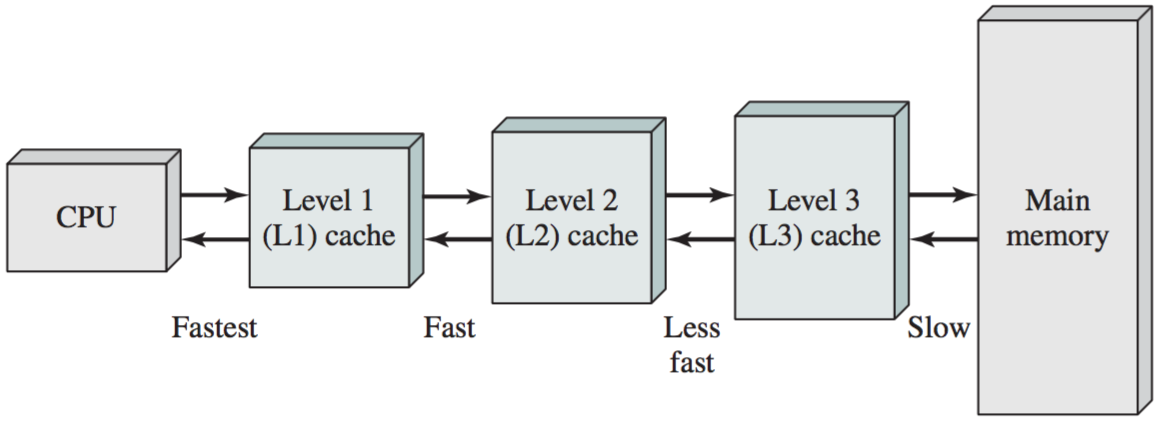
\includegraphics[width=0.9\textwidth]{images/caches.png}
\end{center}

The effective access time formula needs to be updated and expanded.

\end{frame}

\begin{frame}
\frametitle{Darn, Missed Again}

If we have a miss in the L1 cache, the L2 cache is checked. 

If the L2 cache contains the desired page, it will be copied to the L1 cache and sent to the CPU. 

If it is not in L2, then L3 is checked. 

If it is not there either, it is in main memory and will be retrieved from there and copied to the in-between levels on its way to the CPU. 

Because caches have limited size, we have to manage this storage carefully.


\end{frame}

\begin{frame}
\frametitle{Page Replacement Algorithms}

Whenever a page fault occurs, the operating system needs to choose which page to \alert{evict} from the cache to make space for the new one. 

This assumes that the cache is full, which it likely is except at system startup. 

We could, of course, just select a random page...\\
\quad We should do this task more intelligently, if we can.

\end{frame}


\begin{frame}
\frametitle{Page Replacement Algorithms}
To make an intelligent decision about what sort of strategy to choose, we need to know a few things about how data is accessed in a system.

A few observations about memory accesses:

\begin{enumerate}
	\item A rule of thumb in software engineering: the 90/10 rule.
	\item The principle of \alert{temporal locality}. 
	\item The principle of \alert{spatial locality}.
\end{enumerate}

\end{frame}

\begin{frame}
\frametitle{Temporal \& Spatial Locality}

Example: a function that sums up all the values of an array. 

The sum variable is accessed repeatedly, and the fact that it was recently accessed means it is likely to be accessed again soon. 

The array being accessed at index $i$ now means it is likely that the array at index $i+1$ is likely to be accessed soon.

\end{frame}

\begin{frame}
\frametitle{Writing It Out}

If a page has been altered in cache, then that change has to be written to main memory at some point. 

It can be done immediately when the page is changed, or it can be done when the page is evicted from the cache. 

The second option means fewer main memory accesses, if a page is written to multiple times before it is sent to main memory.

If that memory is shared, however, between multiple processors or an I/O device, then the delay in updating main memory may be intolerable. 

\end{frame}

\begin{frame}
\frametitle{Writing It Out}


If a page has not been modified in cache, it can simply be overwritten. 

If all other factors are equal, we should replace a page that has not been modified, as the work to write it out to memory need not be done.

Just overwrite it with the new one!

\end{frame}

\begin{frame}
\frametitle{The Optimal Algorithm}

The optimal algorithm is simple: replace the page that will be used most distantly in the future. 

For each page, make a determination about how many instructions in the future that page will be accessed. 

The selected page is the one with the highest value.


\end{frame}

\begin{frame}
\frametitle{The Optimal Algorithm}

Unfortunately, there is a glaring flaw: it is impossible to implement. 

It requires clairvoyance, and, at least as far as I know, nobody has invented a way to do so reliably. 

The program and OS have no real way of knowing which pages will be used in the future; they can only guess.

\end{frame}

\begin{frame}
\frametitle{The Optimal Algorithm}

It is unimplementable so why talk about it?

It is mostly a benchmark against which other algorithms can be compared. 

Suppose an algorithm is, say, 1\% less efficient than the hypothetical optimal.

No matter how much we improve it, the max performance increase is 1\%.


\end{frame}

\begin{frame}
\frametitle{Not Recently Used}

Operating systems may collect page usage statistics. 

If so, we may have two status bits associated with each page, called $R$ and $M$.

The $R$ bit is set when a page is referenced (either read or written).\\
The $M$ bit is set when the page is written to (modified). 

Once a bit is set, it remains so until the OS changes its value. 


\end{frame}

\begin{frame}
\frametitle{NRU, $R$, and $M$}

The $R$ and $M$ bits can used to build a paging algorithm.

Initially, $R$ and $M$ are 0. 

Periodically, the $R$ bit is cleared to identify pages not recently referenced. 

This may happen every clock interrupt, for example.

\end{frame}


\begin{frame}
\frametitle{NRU Replacement}

Examine all the pages and sort them into 4 buckets based on the $R$ and $M$ bits:

\begin{enumerate}
	\item Not referenced, not modified.
	\item Not referenced, modified.
	\item Referenced, not modified.
	\item Referenced, modified.
\end{enumerate}

Prefer to to remove a page from the lowest-numbered class, when possible. 

\end{frame}

\begin{frame}
\frametitle{First-In-First-Out}

First-In-First-Out is quite easy to understand and implement. 

Some sort of temporal locality. 

If there are $N$ frames, keep a counter that points to the frame that is to be replaced (the counter ranges from $0$ to $N-1$). 

Whenever a page needs to be replaced, replace the page at the counter index and increment the counter (wrap around to 0).


\end{frame}

\begin{frame}
\frametitle{FIFO Replacement}

Some of the time this strategy works. 

If a page is not going to be referenced again (or at least, for a very long time), it is a good choice to get rid of. 

Often times, however, the same page is referenced repeatedly, and this algorithm does not take that into account. 

If a page is referenced often, we want to keep it in memory, not evict it just because it has been in the cache the longest. 

So FIFO is probably not the best choice.

\end{frame}

\begin{frame}
\frametitle{A Second Chance (The Clock)}

Attempt to improve on the FIFO algorithm.

Give pages a ``second chance'' based on the $R$ bit.

If the oldest page's $R$ bit is not set, then the oldest page is removed. 

If the oldest page has recently been referenced, the R bit is cleared.

\end{frame}

\begin{frame}
\frametitle{A Second Chance}

The search then goes to the next-oldest page and repeats the procedure. 

This happens until a page is removed. 

Because the algorithm clears the $R$ bit as it goes, even if all pages have recently been referenced, eventually a page will be selected and evicted. 

Thus the algorithm will eventually terminate. 

\end{frame}

\begin{frame}
\frametitle{A Second Chance}

The index is updated whenever this happens so a page that got a second chance is not the ``oldest'' anymore. 

In some textbooks this is called the Clock replacement algorithm because we can think of the cache as a circular buffer.

The current oldest page is depicted being pointed to by the hand of the clock.

\end{frame}

\begin{frame}
\frametitle{Least-Recently-Used}

The least recently used (LRU) algorithm means the page that is to be replaced is the one that has been accessed most distantly in the past. 

You might consider time stamps and searching a list.

Because there are only two operations, it need not be that complex. 

When a page in the cache is accessed, move that page to the back of the list.

Evict the page at the front of the list.

\end{frame}

\begin{frame}
\frametitle{LRU}

This requires nothing more than a cyclic doubly-linked list. 

Both operations can be performed in $\Theta(1)$ time.

\begin{center}
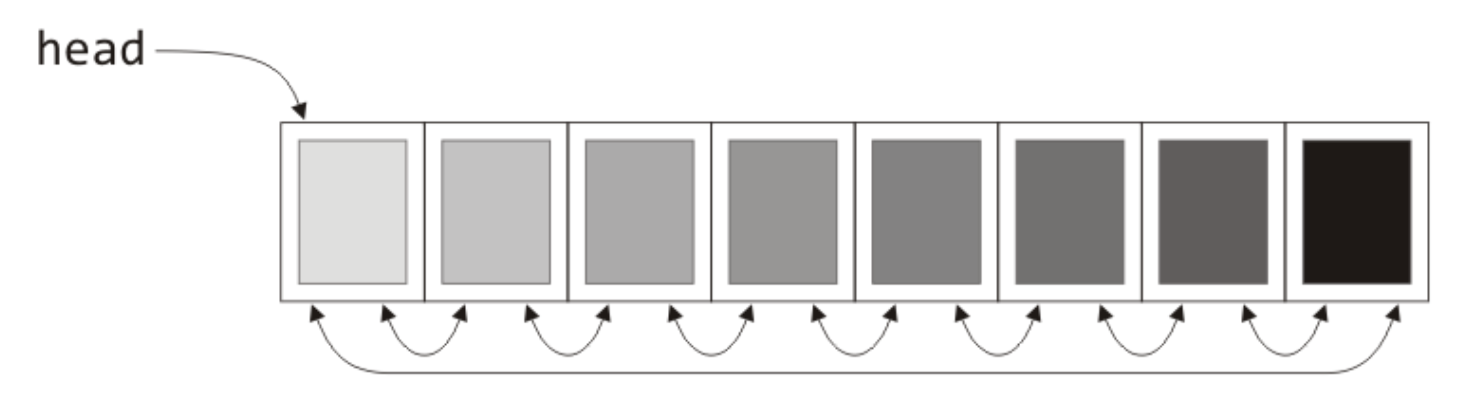
\includegraphics[width=\textwidth]{images/lru-linkedlist.png}
\end{center}


\end{frame}

\begin{frame}
\frametitle{Not Frequently Used}

The not frequently used (NFU) algorithm is similar to the LRU approach.

It can be implemented in software rather than relying on hardware support.

Each page gets an associated software counter, which starts at 0. 

Whenever the $R$ bit would have been updated to 1, 1 is added to the counter. 

When a page is to be replaced, evict the page with the lowest counter value.

\end{frame}

\begin{frame}
\frametitle{NFU = Never Forgets ... Uh... Usage?}

NFU never forgets and counters can never decrease. 

A page that was accessed very frequently at the start of the program will accumulate a high counter value early on, and therefore might never be evicted.

Even if it is not needed again. 

What we need is a way for the count to decline over time. 



\end{frame}

\begin{frame}
\frametitle{NFU: Aging}

\alert{Aging}: counters are shifted to the right by 1 bit before the 1 is added.\\
\quad Instead of adding 1 set the leftmost bit to 1. 

Now we have a bit array of byte size.

A page that has not been referenced in a while has its value decrease over time. 

We still evict the lowest value page when it is time to replace a page.

\end{frame}

\begin{frame}
\frametitle{Aging has its Disadvantages}

We lose a certain amount of precision compared to the LRU approach.

If pages $a$ and $b$ both have patterns of \texttt{00000001} we know they were both last accessed 8 cycles ago. 

All history before that point is lost. 

Which page between $a$ and $b$ was least recently used is unknown.


\end{frame}

\begin{frame}
\frametitle{Pre-Paging}

Thus far all strategies for putting things in the cache have been ``on-demand''.
 
Suppose instead that the OS guesses what pages might be needed next.

This might reduce the amount of time spent waiting for a page in the future.

\end{frame}

\begin{frame}
\frametitle{Pre-Paging}

Predicting which pages are likely to be used in the near future is, indeed, a matter of clairvoyance. 

There exist various techniques to determine the likely pages to be used frequently (called the ``working set'').

They are complex and will not be examined further right now.

\end{frame}

\begin{frame}
\frametitle{Pre-Paging: Startup}

A situation in which pre-paging might be useful is when a program is started or swapped into memory. 

Technically, no pages of the process need to be loaded into the cache to start with; we can simply suffer through a whole bunch of page faults. 

This is rather slow; it might be better to load multiple pages into the cache.

This will of course require some guesses about what pages will be needed.

\end{frame}

\begin{frame}
\frametitle{Paging Overview Summary}

A quick overview of the algorithms we have discussed:

\begin{center}
\begin{tabular}{l|l}
	\textbf{Algorithm} & \textbf{Comment} \\ \hline
	Optimal & Impossible to implement; a benchmark\\
	Not Recently Used &  Not very good performance \\
	First In First Out & Highly suboptimal \\
	Second Chance & Much better than FIFO, but just adequate \\
	Least Recently Used & Best performer, difficult to implement? \\
	Not Frequently Used & Approximation of LRU \\
	NFU + Aging & Better approximation of LRU\\
\end{tabular}
\end{center}


\end{frame}

\begin{frame}
\frametitle{Local and Global Replacement}

When a process switch occurs, we could dump the entire cache to make way for the next process to run, but this is most likely unnecessary work. 

If $P_{1}$ is suspended now, $P_{2}$ may run for a while and then $P_{1}$ runs again.

It may be that when $P_{1}$ starts again, some of its pages are still in the cache.

If $P_{2}$ did replace all the cache lines, that is the worst case scenario. 

So we may have multiple processes with pages in the cache at a given time.

\end{frame}

\begin{frame}
\frametitle{Local and Global Replacement}

Should care about which process a victim page belongs to or not? 

Suppose we are using the LRU algorithm. 

If process $P_{1}$ has a page fault, do we replace the least recently used page in all the cache (global replacement)? 

Or do we replace the least recently used page in the cache that belongs to $P_{1}$ (local replacement)?


\end{frame}

\begin{frame}
\frametitle{Think Globally; Act Locally}

Of course, different levels of cache might have different strategies. 

If the L1 cache is 16~KB and pages are 4~KB, there can be 4 pages in the L1 cache, so global replacement probably makes sense there. 

If L2 cache is 256~KB there are 64 pages and maybe local replacement makes sense there, but even 64 pages is fairly small.

When caches are somewhat larger, however, things may be more interesting.

\end{frame}


\begin{frame}
\frametitle{Local and Global Replacement}

Local algorithms give each process some fixed number of pages in the cache. 

Global algorithms dynamically allocate cache space to different programs based on their needs; the number of pages in the cache for each process varies.

Global algorithms allegedly work better, when processes' memory needs change over time.

If the local algorithm is used, we may be wasting some of the space in the cache for a process that does not really need it right now. 

\end{frame}

\begin{frame}
\frametitle{Page Fault Frequency}

Suppose we have a large cache, and a dynamic allocation (global algorithm).

We want some intelligence to keep any process from having too many or too few pages in the cache. 

To manage the complexity of how much of the cache should be allocated to a particular process, we might wish to keep track of the number of page faults.

The measure is called the \alert{page fault frequency} or PFF. 


\end{frame}

\begin{frame}
\frametitle{Page Fault Frequency}

In simplest terms, the PFF is the guide for telling whether a given process has too few, too many, approximately the right number of pages. 

PFF too high? More cache space is needed for that process. 

PFF low? The process has too much cache space allocated.

Note: relies on assumption that more cache space means fewer page faults.\\
\quad This is true for LRU, but not necessarily for FIFO!

\end{frame}

\end{document}

